  % !TEX encoding = UTF-8 Unicode
\documentclass[a4paper]{article}

\usepackage{color}
\usepackage{url}
%\usepackage[T2A]{fontenc} % enable Cyrillic fonts
\usepackage[utf8]{inputenc} % make weird characters work
\usepackage{graphicx}

\usepackage[english,serbian]{babel}
%\usepackage[english,serbianc]{babel} %ukljuciti babel sa ovim opcijama, umesto gornjim, ukoliko se koristi cirilica

\usepackage[unicode]{hyperref}
\hypersetup{colorlinks,citecolor=green,filecolor=green,linkcolor=blue,urlcolor=blue}

\usepackage{listings}

%\newtheorem{primer}{Пример}[section] %ćirilični primer
\newtheorem{primer}{Primer}[section]

\definecolor{mygreen}{rgb}{0,0.6,0}
\definecolor{mygray}{rgb}{0.5,0.5,0.5}
\definecolor{mymauve}{rgb}{0.58,0,0.82}

\lstset{ 
  backgroundcolor=\color{white},   % choose the background color; you must add \usepackage{color} or \usepackage{xcolor}; should come as last argument
  basicstyle=\scriptsize\ttfamily,        % the size of the fonts that are used for the code
  breakatwhitespace=false,         % sets if automatic breaks should only happen at whitespace
  breaklines=true,                 % sets automatic line breaking
  captionpos=b,                    % sets the caption-position to bottom
  commentstyle=\color{mygreen},    % comment style
  deletekeywords={...},            % if you want to delete keywords from the given language
  escapeinside={\%*}{*)},          % if you want to add LaTeX within your code
  extendedchars=true,              % lets you use non-ASCII characters; for 8-bits encodings only, does not work with UTF-8
  firstnumber=1000,                % start line enumeration with line 1000
  frame=single,	                   % adds a frame around the code
  keepspaces=true,                 % keeps spaces in text, useful for keeping indentation of code (possibly needs columns=flexible)
  keywordstyle=\color{blue},       % keyword style
  language=Python,                 % the language of the code
  morekeywords={*,...},            % if you want to add more keywords to the set
  numbers=left,                    % where to put the line-numbers; possible values are (none, left, right)
  numbersep=5pt,                   % how far the line-numbers are from the code
  numberstyle=\tiny\color{mygray}, % the style that is used for the line-numbers
  rulecolor=\color{black},         % if not set, the frame-color may be changed on line-breaks within not-black text (e.g. comments (green here))
  showspaces=false,                % show spaces everywhere adding particular underscores; it overrides 'showstringspaces'
  showstringspaces=false,          % underline spaces within strings only
  showtabs=false,                  % show tabs within strings adding particular underscores
  stepnumber=2,                    % the step between two line-numbers. If it's 1, each line will be numbered
  stringstyle=\color{mymauve},     % string literal style
  tabsize=2,	                   % sets default tabsize to 2 spaces
  title=\lstname                   % show the filename of files included with \lstinputlisting; also try caption instead of title
}

\begin{document}

\title{Etika u računarstvu\\ \small{Seminarski rad u okviru kursa\\Metodologija stručnog i naučnog rada\\ Matematički fakultet}}

\author{
	Marina Borozan, Matija Miličević,\\
	Stefan Mirić, Nikola Vuković\\
	marinaborozanv@gmail.com, matijanme@gmail.com,\\
	stefangiggs96.sm@gmail.com, sterlu.sd@gmail.com
}

%\date{9.~april 2015.}

\maketitle

\abstract{
  Sažetak rada, kao reklama za rad. Jedan pasus, piše se na kraju. 
}

\tableofcontents

\newpage

\section{Uvod}

Uvod u temu, definisanje pojmova, cilj rada, najava ostatka rada.
Pisati pred kraj, pre apstrakta. Treba da sadrži reference.

\section{Etika}
Etika se definiše kao oblast filozofije koja se bavi sistematizacijom, odbranom i preporukom ispravnog i pogrešnog ponašanja. Često se uvodi podela na metaetiku, normativnu etiku i primenjenu etiku \cite{ethics-iep}. 

Metaetika se bavi proučavanjem temelja etike, načina na koje definišemo pojmove, kao i njihovim stvarnim značenjem. Može se posmatrati kao visokoapstraktno filozofsko razmišljanje o moralnosti \cite{metaethics-iep}. Postavlja apstraktna pitanja kao ``Šta je dobrota?'' i ``Odakle dolaze naše moralne vrednosti?''.

Normativna etika se bavi praktičnim načinima definisanja pravilnog i pogrešnog. Ova grana etike nam je najkorisnija kada razmatramo moralne probleme u računarstvu i njihove implikacije, pa ćemo se njom najviše i baviti. 

Primenjena etika se bavi razmatranjem konkretnih kontroverznih situacija i pitanja moralnog karaktera. Deli se na mnogo podgrana koje proučavaju situacije specifične za određene oblasti. U osnovi se svodi na primenu principa definisanih u teorijama normativne etike. Međutim zaplet nastaje kada različite teorije daju suprotne odgovore. 

\section{Teorije etike}
Svaka teorija etike sadrži dva obavezna elementa. Prvi je teorija koja definiše šta se smatra za dobro, odnosno vredno. Za definisanje pojma ``dobro'' teorija etike može uzeti bilo koji pojam za koji se zalaže (na primer lična sloboda ili život svih ljudi). Ipak često nije dovoljno definisati samo ovaj pojam da bi se izbegle dileme u izboru pravilnog postupka. Zato se uvek definiše i teorija ispravnog koja nalaže kako pojedinci treba da reaguju na vrednosti. 

Osvrnućemo se na neke škole etike i njihove dobre i loše strane. Pregled koji sledi nikako ne predstavlja pregled svih grana etike koji bi bio preopširan, već služi da čitaocu da ideju o različitim pristupima definisanja dobrog i ispravnog. 

\begin{table}[h!]
\begin{center}
\caption{Pregled teorija etike i vrednosti koje zastupaju}
\begin{tabular}{|c|c|c|} \hline
Etika vrline & Deontologija & Konsekvencijalizam\\ \hline
Delatnik & Delo & Posledice\\ \hline
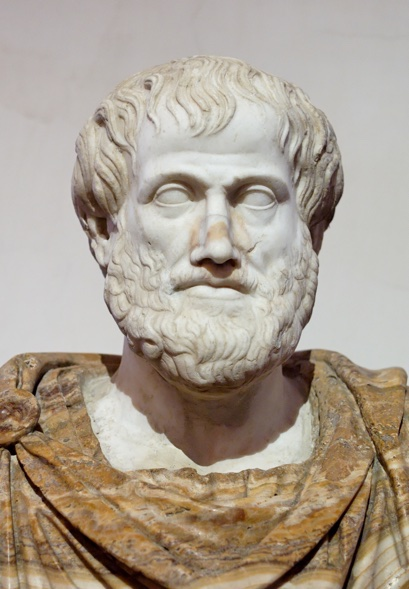
\includegraphics[scale=.2]{slike/aristotel.jpg} & 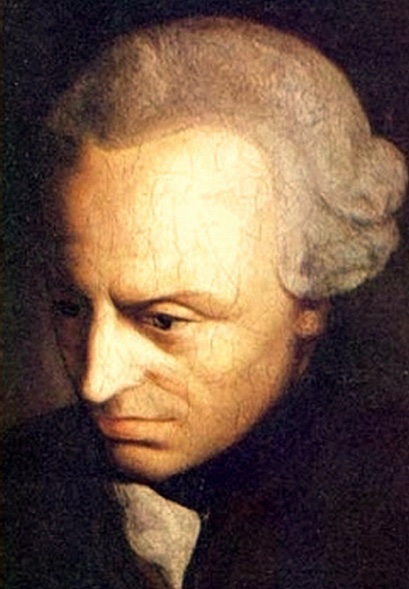
\includegraphics[scale=.2]{slike/kant.jpg} & 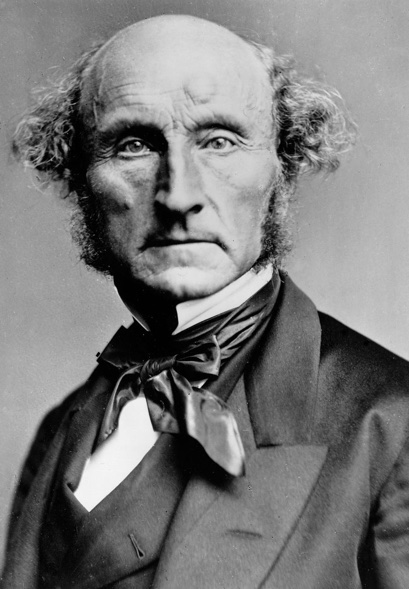
\includegraphics[scale=.2]{slike/mil.jpg} \\Aristotel & Imanuel Kant & Džon Stjuart Mil\\ 384-322 PNE & 1724-1804 & 1806-1873\\ \hline \end{tabular}
\label{tab:tabela1}
\end{center}
\end{table}

\subsection{Etika vrline}

Etika vrline zastupa moralnost samog delatnika u datoj situaciji. 

Koren u antičkoj Grčkoj - Platon i Aristotel

(virtue ethics)

\subsection{Deontologija}
Deontologija, ili nekad teorija dužnosti, zastupa poštovanje vrednosti iznad svega drugog, uključujući i posledice. 
Termin deontologija potice od grčkih reči koje označavaju dužnost (deon) i nauku (logos). Prema savremenoj moralnoj filozofiji, deontologija spada u domen moralnih teorija koje procenjuju moralnost postupaka(izbora), tj. procenjuje se ono sto je ispravno učiniti, pa se tako izbori mogu klasifikovati kao moralno obavezni, dozvoljeni ili zabranjeni. Za razliku od ovih teorija, etika vrline procenjuju kakva osoba bi trebalo da budemo i u skladu sa tim da delujemo. 

(Kantijanizam - Kantianism)

\subsection{Konsekvencijalizam}
Konsekvencijalizam prema savremenoj moralnoj filozofiji tvrdi da se izbori(postupci) mogu moralno proceniti samo po njihovim posledicama - krajnjim ishodima. Prema ovom tvrdjenju, ukoliko izbor zajedno sa svim njegovim posledicama uvećava kolektivno dobro, taj izbor je moralno napraviti.

(Utilitarizam postupaka - Act utilitarism)

(Utilitarizam pravila - Rule utilitarism)

(social contract theory)

\subsection{Poredjenje deontologije i konsekvencijalizma}
U domenu moralnih teorija koje procenjuju izbore, deontolozi su suprotstavljeni konsekvencijalistima, pa ćemo uporedno prikazati neke aspekte oba pravca.

Poznati primer konsekvencijalizma je problem transplantacije. Ukoliko hirurg moze da spasi od sigurne smrti pet pacijenata kojima je potrebna transplantacija organa, prema konsekvencijalizmu, on ima pravo (prema nekima i moralnu obavezu) da ubije jednog zdravog pacijenta i uzme njegove organe. Podrazumeva se da su bitne posledice samo preživljavanje pet pacijenata i smrt jednog.
Jedna od prednosti deontološkog pristupa je da se ubijanje, maltretiranje ili oduzimanje materijalnih dobara od nevinih pojedinaca smatra nemoralnim, čak i kada posledice toga mogu uvećati kolektivno dobro. Zbog toga sto konsekvencijalizam zastupa obrnut stav, često je kritikovan u savremenoj moralnoj filozofiji.

Kada je reč o konfliktnim izborima, konsekvencijalizam jasno odlučuje koji je moralno napraviti - onaj koji zajedno sa posledicama proizvodi više dobrog. Medjutim, deontolozi se mogu naci u dilemi ukoliko su oba izbora moralno ispravna, a medjusobno konfliktna. Stoga, iako izgleda kontraintuitivan, konsekvencijalizam nekad ima objašnjenja za brojne deontoloske moralne dileme.

Takodje, deontologija ne zahteva da pravimo takve lične izbore koji bi uvek imali dobre ishode i za druge. 


\section{Odnos etike i tehnološkog razvoja}

Etika je kao naučna disciplina postojala pre mnogih tehnoloških napredaka civilizacije. Kako su mogućnosti pojedinaca ili grupa rasle tako je dolazilo i do novih etičkih pitanja. Naučni razvoji u fizici i hemiji su bez sumnje doveli do poboljšanja uslova života mnogima, ali moramo biti svesni mogućnosti novih tehnologija. Primer: ``Da li je etički koristiti biološko ili nuklearno oružje u ratu?''.

Pojavom ličnih računara i interneta mnogima je pružena mogućnost da komuniciraju na velikim daljinama, vrše monetarne transakcije, dele multimedijski sadržaj... Međutim, time je takođe olakšano lažno predstavljanje, prevara, deljenje neovlašćenog sadržaja i slično ,na načine ne prethodno viđene.
Kao što vidimo tehnološki napredak uvodi nove etičke izazove.

Jedna od oblasti etike koja je usko vezana za računarsku etiku je etika tehnologije. Pomenućemo neke od popularnijih stavova vezanih za etiku tehnologije:
\begin{itemize}
	\item \textbf{Tehnicizam} -
	Mišljenje da je tehnologija korisna kao alat i da njenom upotrebom možemo da unapredimo ljudsko društvo. Ideja je da jednog dana ljudi će moći rešiti sve praktične probleme koriščenjem tehnoloških alata i metoda.
	\item \textbf{Optimizam} - Verovanje da tehnologija pozitivno utiče na ljudsko društvo i da je moralno dobra. Za razliku od tehnicizma ovde tehnologija nije samo alat već je usko povezana sa identitetom čoveka.
	\item \textbf{Skepticizam} - Mišljenje da tehnološki napretci čine štetu društvu.
	Kako društvo napreduje tehnološki, tako i nazaduje u slobodi i psihičkom blagostanju.
\end{itemize}


\section{Etika i računari}

Računarska etika se pojavljuje prvi put 1940-ih u radu profesora MIT-a
Norberta Vinera (Norbert Wiener)\cite{bynum}. Viner je za vreme Drugog svetskog rata radio na razvoju elektronskih računara i drugih informacionih tehnologija. U tom periodu je zajedno sa svojim kolegama stvorio novu granu nauke, ``kibernetiku'', koja se bavila regulatornim sistemima, odnosno komunikacijom i međusobnom kontrolom delova sistema koji sami sebe regulišu.
Nakon završetka rata napisao je knjigu ``Kibernetika''(1948) u kojoj je opisao novonastalu oblast i pomenuo neke društvene i etičke implikacije elktronskih računara. Dve godine nakon toga je izdao novu knjigu, ``Ljudska upotreba ljudskih bića''(1950) u kojoj je istražio veliki broj etičkih problema koji bi verovatno nastali napretkom informacionih tehnologija. Na taj način on je postavio temelje za modernu etiku računarstva, baveći se pitanjima poput: računarske bezbednosti, računarskih mreža i globalizacije, robotske etike, veštačke inteligencije, etičkih dužnosti računarskih profesionalaca...

Vinerov rad se pokazao toliko naprednim za svoje vreme, da je sve do 1976. godine bilo malo pomaka u polju računarske etike. Te godine profesor Volter Maner (Walter Maner) je primetio da etički problemi na njegovom kursu medicinske etike budu teži ili se uveliko menjaju u slučajevima kada se računari pridodaju. Njemu je delovalo da se uz računare pojavljuju etički problemi koji nebi postojali da nije bilo izuma elktronskog računara. Posmatrajući ovu pojavu došao je do zaključka da bi trebala postojati nova grana primenjene etike, poput medicinske i poslovne etike. Odlučio je da tu novu granu nazove ``Računarska etika''. Bitno je pomenuti da, iako se bavio mnogim pitanjima računarske etike, Norbert Viner nije koristio termin računarska etika. Takođe Maner nije bio svestan postojanja Vinerovih radova o kibernetici.

Maner je zatim kreirao eksperimentalni kurs računarske etike namenjen za studente informatike. Eksperiment je bio uspešan i usled visoke potražnje Maner je konstruisao plan za kurs računarske etike 1978. godine. Narednih godina je držao radionice i govore po konferencijama, sve do 1980. godine kada je njegov koncept kursa izdat u vidu monografa, koji je imao sve informacije neophodne za držanje nastave. Na ovaj način je došlo do popularizacije računarske etike u akademskoj zajednici, najviše u oblastima filozofije i računarstva.



\subsection{Vidjenja računarske etike}
``Računarska etika'' kao termin nema opšte prihvaćenu definiciju. Usled brzog razvoja informacionih tehnologija došlo je do toga da teorija računarske etike često kasni za praktičnim problemima novih tehnologija. Zbog ovoga se mnogi ti problemi rešavaju individualno \textit{ad hoc} metodama, na primer analogijom na slične probleme, umesto stvaranja novog teorijskog okvira za rešavanje takvih problema. Ovakav pristup je doveo do određenih nesuglasica i mnogi autori se ne slažu kako tačno treba posmatrati ovu oblast. Postavlja se pitanje u kojoj meri je računarska etika precizno određena oblast, a u kojoj meri nasumična kolekcija praktičnih problema i rešenja.

U naučnoj literaturi se može pronaći pet pristupa računarskoj etici\cite{floridi}:

\begin{enumerate}
	\item \textbf{} (No resolution approach) -
	\item \textbf{} (The professional approach) -
	\item \textbf{} (The radical approach) -
	\item \textbf{} (The conservative approach) -
	\item \textbf{} (The innovative approach) -
\end{enumerate}



%\subsection{Apstraktna priroda računarskog sveta}
%Pored samog hardvera, u pojam računara često uključujemo i softver, sačuvane podatke, veze tog računara sa drugim računarima i slično. Možemo da vidimo da ako želimo da se bavimo računarskom etikom moramo da posebno obratimo pažnju i na apstraktne aspekte računara.


\subsection{Računarske mreže i tipovi interakcija}
Pored toga što su računari sami po sebi kompleksni, oni se mogu povezati u mrežu čime se omogućava međusobna interaktivnost. Ovako umreženi računari mogu da dele informacije među sobom, postižući veću funkcionalnost, po ceni rizika eventualnih napada od strane trećeg lica. Ovo dovodi do etičkih pitanja vezanih za naš pristup tuđim ili tuđi pristup našim računarima. Postavlja se pitanje kada i koji tipovi interakcije su etički pri pristupu tuđem uređaju.

%priča o belim, sivim, crnim hakerima. Ne detalji samo ukratko i o etici

\section{Primeri etičkih dilema u računarstvu}

%Da bi možda bilo jasnije kakvim se to tačno dilemama bavi Računarska etika, posmatraćemo nekoliko konkretnih primera.
Da bi možda bilo jasnije kakvim se to tačno dilemama bavi računarska etika, čitaocima ćemo predstaviti detaljno jedan primer iz stvarnog sveta. Takođe ćemo pomenuti još nekoliko aktuelnih etičkih pitanja.

\subsection{Primer: Pisanje virusa}
Jedan od velikih dilema računarske bezbednosti je vezan za edukaciju studenata o pisanju računarskih virusa(eng. \textit{malicious code, malware}).

U prilog odričnom odgovoru idu argumenti tipa ``Zašto bi učili studente nečemu sto je loše'', dok u suprotnom idu odgovori ``Treba ih učiti da bi znali da
naprave i primene sisteme odbrane od virusa''.

Uopšteno govoreći, treba odgovoriti na tri pitanja:
\begin{enumerate}
	\item Kako ćemo studente učiti o temi računarskih virusa i zlonamernog koda uopšte?
	\item Da li ih možemo učiti, a da to bude korisno, upotrebljivo, ali i bezbedno?
	\item Da li će odabrani način učenja učiniti ovaj svet boljim ili lošijim?
\end{enumerate}

Na univerzitetu u Kalgariju (eng. \textit{Calgary}) 2003. godine profesor Ken Barker odlučio je da u sklopu kursa koji se odnosi na računarsku sigurnost, njegovi
studenti treba da nauče da pišu viruse. Nasuprot nadanjima fakulteta, antivirusne kompanije su veoma negativno reagovale na ovakav potez.
On je ovako objasnio svoju ideju: ``Kurs je o razumevanju virusa, kako bi se isti zaustavili.
Želimo da stvorimo sledeću generaciju antivirusnih profesionalaca koji će se boriti sa sledećom generacijom virusnog softvera''.
Studenti bi na kursu radili u obezbeđenim računarskim laboratorijama, tako da virusi ne bi stigli do Interneta, takođe ne bi pisali nove viruse nego 
bi prepravljali već postojeće.

``Potrebni su nam dobri momci koji će razmišljati kao loši momci. Potrebni su nam ljudi koji će unapred otkrivati nove pravce napada i nove ranjivosti i razvijati vakcine pre nego što se virus i pojavi.
Bolje je da imamo antivirusnu zajednicu koja će misliti jedan korak unapred i koja će pokušavati da shvati šta će sledeći potez biti i blokirati ga, nego da čekamo da loši momci naprave prvi korak''
rekao je Barker i bez obzira na negativne kritike, nastavio je sa svojom idejom.

Kako je pisati virus dosta jednostavnije nego otkriti i blokirati ga,jasna je zabrinutost da se ne zloupotrebi stečeno znanje, a takođe ljudi koji vide da univerzitet Kalgari predaje i podržava pisanje virusa i pomisliće da je to u redu. 
To ohrabruje pisce virusa i daje im legitimnu notu.

Profesor računarstva na Sonoma univerzitetu Džordž Ledin (George Ledin) osnovao je kurs kako bi podučili studente kako da naprave bolju sigurnosnu zaštitu.Sigurnosne kompanije,s druge strane, su osuđivale
svaki pokušaj da se stvori novi zlonamerni program, bezobzira na njegov cilj. Iako je jasno naglasio da je plan da se studenti poduče da prave viruse u kontrolisanom okruženju u svrhu podučavanja, kako da
ih spreče i unište, barem tri kompanije su poslale pismo Ledinu u kojem su najavili bojkot njegovih studenata.
Njegov odgovor na novinarske članke, u kojima se poprilično kritikuje njegova edukacija o virusima, bio je: ``Studenti informatike moraju da nauče da prepoznaju, analiziraju, onesposobe i unište zlonamerne programe.
Da bi to umeli, oni moraju da sami shvate kako crvi i virusi funkcionišu. Naravno da postoji mogućnost da oni pređu na tamnu stranu, ali ista opasnost postoji i sa doktorima. Moraćemo da se oslonimo na njihovu etiku''.


Vrlo je interesantno da je opšto mišljenje studenata to da ih treba edukovati o ovoj temi. Verovatno većina ima želju da se oproba u nečemu što je na granici zabranjenog, što svakako nije baš dobar motiv,
dok je takođe popularno mišljenje da su antivirusne kompanije nekako povezane sa pisačima virusa.

\subsection{Dodatni primeri}
%Možda promeniti naziv podglave
Još neka zanimljiva etička pitanja se npr. odnose na kopiranje-prodaju-distribuciju softvera.
\begin{itemize}
\item Da li je prihvatljivo da se kupi softver pa onda instalirati ga dvaputa?
\item Šta ako ga instaliramo,a onda damo prijatelju da ga koristi?
\item Šta ako ga instaliramo a zatim napravimo 50 kopija i prodamo zainteresovanim kupcima?
\end{itemize}
Zatim,
\begin{itemize} 
\item Da li kompanija ima pravo da čita elektronsku poštu svojih zaposlenih?
\item Da li kompanija ima pravo da nadzire koje Web stranice njeni zaposleni posećuju?
\item Da li pojedinac ima pravo na privatnost podataka?
\item Da li korisnik ima dužnost da poštuje intelektualnu svojinu koja pripada proizvodu - ne modifikujući ga iako je svrha poboljšanje proizvoda?
\end{itemize}

\section{Zaključak}
\label{sec:zakljucak}

Zaključak

\addcontentsline{toc}{section}{Literatura}
\appendix
\bibliography{seminarski} 
\bibliographystyle{plain}

\appendix
\section{Dodatak}
Ovde pišem dodatne stvari, ukoliko za time ima potrebe.


\end{document}

